%!TEX root = ../report.tex

\begin{document}
    \chapter{附加功能}

	
	\section{键鼠交互的相机旋转移动}
	\subsection{平移旋转变换}
	\begin{spacing}{2.5}
	其实,所谓相机的旋转移动可以看成相机固定不动,而物体在进行逆变换,例如,相机左移一个单位其实就是物体向右移动一个单位。因此要相机的旋转移动,只要实现物体对应的旋转移动即可。所用到的变换矩阵如下:
	\begin{enumerate}
		\item 平移变换矩阵
		\begin{equation}
		\begin{pmatrix}
			1 &  0&  0&0 \\ 
 			0&  1&  0& 0\\ 
 			0& 0 & 1 &0 \\ 
 			T_{x}&  T_{y}&  T_{z}& 1
		\end{pmatrix}
		\label{transfer_1}
		\end{equation}
		\item 	绕X轴旋转变换矩阵
		\begin{equation}
		\begin{pmatrix}
			 1&  0&  0 &0 \\ 
 			0&  cos\theta &  sin\theta& 0\\ 
 			 0& -sin\theta & cos\theta &0 \\ 
 			0&  0&  0& 1
		\end{pmatrix}
		\label{yrotate}
		\end{equation}
		\item 绕Y轴旋转变换矩阵
		\begin{equation}
		\begin{pmatrix}
			cos\theta &  0&  -sin\theta &0 \\ 
 			0&  1&  0& 0\\ 
 			sin\theta & 0 & cos\theta &0 \\ 
 			0&  0&  0& 1
		\end{pmatrix}
		\label{xrotate}	
		\end{equation}
	
		\item 绕Z轴旋转变换矩阵
		\begin{equation}
		\begin{pmatrix}
			cos\theta &  sin\theta &  0 &0 \\ 
 			-sin\theta &  cos\theta &  0& 0\\ 
 			0 & 0 & 1 &0 \\ 
 			0&  0&  0& 1
		\end{pmatrix}
		\label{zrotate}
		\end{equation}
		\item 缩放变换矩阵
		\begin{equation}
		\begin{pmatrix}
			S_{x}& 0 &  0 &0 \\ 
 			0 &  S_{y} &  0& 0\\ 
 			0 & 0 & S_{z} &0 \\ 
 			0&  0&  0& 1
		\end{pmatrix}
		\label{zrotate}
		\end{equation}
	\end{enumerate}
	\end{spacing}

	\subsection{键鼠交互}
\begin{spacing}{2.5}
		为了增加交互性,我们自己加入了键鼠交互方面的功能,即:键盘通过上下左右或WASD键可以进行视角的移动、通过TAB可以切换场景,鼠标通过拖动也可以实现视角的移动,这些移动本质上是通过物体坐标的改变来实现的\\
	首先需要一个全局事件监听函数,响应event并判断对应的类型,最后执行特定功能函数:
\end{spacing}

	\begin{lstlisting}
void App::OnEvent(SDL_Event* event , double dt)
{
	switch (event->type)
	{
		case SDL_QUIT:
			running = false;
			break;

        case SDL_MOUSEBUTTONDOWN:
            mouseIsDown = 1;
            break;

        case SDL_MOUSEBUTTONUP:
            mouseIsDown = 0;
            break;
        
        case SDL_MOUSEMOTION:
            if(mouseIsDown){
                onMouseDrag(*event);
                break;
            }
            break;

		case SDL_KEYDOWN:
            onKeyPress(event->key.keysym.sym , dt);
            break;
        
		default:
			break;
	}
}
	\end{lstlisting}
	\begin{spacing}{2.5}
			键盘的监听可以使用SDL2库中的键盘事件接口来实现:
	\end{spacing}

\begin{lstlisting}
void App::onKeyPress(SDL_Keycode keyCode , double dt) {
    auto camera = Camera::getInstance();
    auto v = 45;
    auto velo = camera->getMoveVelo();
    switch (keyCode) {
        case SDLK_ESCAPE:
            running = false;
            break;
        case SDLK_w:
            camera->offsetPosition(camera->forward() * velo * dt);
            break;
        case SDLK_s:
            camera->offsetPosition(-camera->forward() * velo * dt);
            break;
        case SDLK_a:
            camera->offsetPosition(-camera->right() * velo * dt);
            break;
        case SDLK_d:
            camera->offsetPosition(camera->right() * velo * dt);
            break;
        case SDLK_z:
            camera->offsetPosition(camera->up() * velo * dt);
            break;
        case SDLK_x:
            camera->offsetPosition(-camera->up() * velo * dt);
            break;
        case SDLK_UP:
            camera->offsetDirection(v * dt, 0);
            break;
        case SDLK_DOWN:
            camera->offsetDirection(-v * dt, 0);
            break;
        case SDLK_LEFT:
            camera->offsetDirection(0, -v*dt);
            break;
        case SDLK_RIGHT:
            camera->offsetDirection(0, v *dt);
            break;
        case SDLK_TAB:
            Camera::getInstance()->resetCamera();
            Canvas::getInstance()->addScene();
            Canvas::getInstance()->resetNode();
            break;
        default:
            break;
    }
}
\end{lstlisting}

	\begin{spacing}{2.5}
			鼠标的监听则要复杂一些,因为要实现拖动的交互效果,SDL2中并没有直接的接口,需要先通过MouseIsDown进行判断,如果鼠标被按下,则调用MouseMotion监听鼠标移动轨迹,通过方向、速率等参数传达到移动函数中,最后调整一些参数,使得拖动效果看起来更真实
	\end{spacing}

\begin{lstlisting}
void App::onMouseDrag(SDL_Event& event) {
    auto v = 45;
    auto camera = Camera::getInstance();
    auto velo = camera->getMoveVelo();
    camera->offsetPosition(camera->right() * velo * event.motion.xrel * 0.001);
    camera->offsetPosition(-camera->up() * velo * event.motion.yrel * 0.001);
    camera->offsetDirection(0 , -v * event.motion.xrel * 0.0028);
    camera->offsetDirection( v * event.motion.yrel * 0.0028, 0);
}
\end{lstlisting}

    \section{区域填充}
    \begin{spacing}{2.5}
    本渲染器用到的区域填充算法是课堂中学过的扫描线填充算法,不同的是这里分了更多情况进行优化分析,在通常情况下,扫描线填充算法运用于一般多边形是比较复杂的,所以项目中我们都采取先转化为三角形单元的形式,但是三角形也分为一般三角形、平底三角形和平顶三角形,后面两种三角形对于扫描线算法而言非常友好,因为其一边可以恰好与扫描线重合。
    对于一般三角形,可以采取从中间分成一个平底三角形和平顶三角形的策略来进行扫描,最后扫描的情况只需要分别针对这两种特殊的三角形即可:
	    \begin{figure}[H]
		\centering
		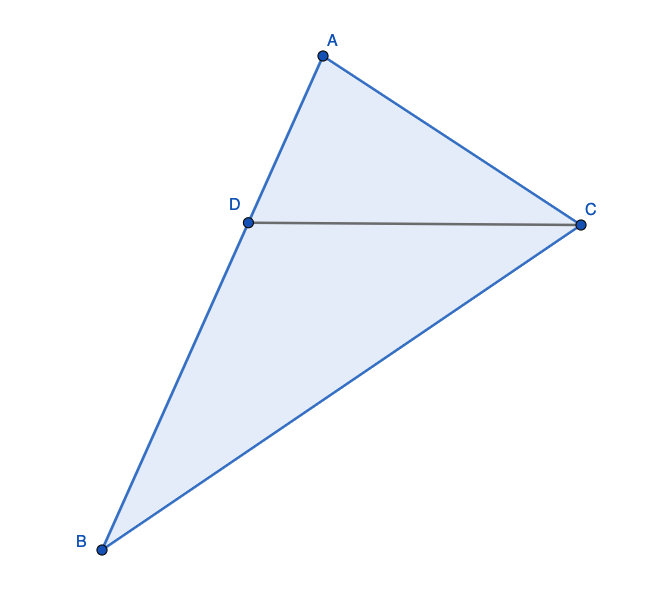
\includegraphics[width=0.6\textwidth]{images/scanline1.png}
		\caption{普通三角形的切分}
		\label{line}
	\end{figure}
	
比如上图的普通三角形ABC,就可以分为一个平底三角形ACD和一个平顶三角形BCD

    \end{spacing}
        \begin{lstlisting}
    if (MathUtil::equal(pVert1->pos.y, pVert2->pos.y)) 
    {
        triangleBottomRasterize(*pVert1, *pVert2, *pVert3);
    }
    else if (MathUtil::equal(pVert2->pos.y, pVert3->pos.y))
    {
        triangleTopRasterize(*pVert1, *pVert2, *pVert3);
    }
    else
    {
        double ty = pVert2->pos.y;
        double factor = (ty - pVert1->pos.y) / (pVert3->pos.y - pVert1->pos.y);
        VertexOut tVert = pVert1->interpolate(*pVert3, factor);
        triangleTopRasterize(*pVert1, tVert, *pVert2);
        triangleBottomRasterize(*pVert2, tVert, *pVert3);
    }

        \end{lstlisting}

    \begin{spacing}{2.5}
    对于平顶三角形而言,扫描线于顶部重合,自顶向下循环遍历y值,通过比例计算插值从而计算出中间情况的需要填充的像素,scanLineFill直接调用底层的drawPixel对像素进行着色
    
    	
    \end{spacing}

	\begin{lstlisting}
    for (int py = startPY; py * sign <= sign * endPY; py = py + sign)
    {
    	double ld = 1.0f;
       	double factor = (py - startPY) * ld / (endPY - startPY);
       	VertexOut vertStart = pVert1->interpolate(*pVert2, factor);
       	VertexOut vertEnd = pVert1->interpolate(*pVert3, factor);
       	scanLineFill(vertStart, vertEnd, py);
   	}
	\end{lstlisting}


    \section{纹理贴图}
    
    \section{光照}
    \begin{spacing}{2.5}
    \subsection{冯氏光照模型}
    现实世界的光照是很复杂的,物体的材质和光照的特性都会影响最终的渲染效果,在有限的计算能力下,我们很难模拟完全真实的光照条件。因此,图形学的渲染更倾向于使用一种简化的模型对现实情况进行近似。\\
    本次我们参考了OpenGL的处理方式,采用冯氏光照模型(Phong Lighting Model)进行光照模拟。冯氏光照模型的主要结构由3个分量组成:环境(Ambient)、漫反射(Diffuse)和镜面(Specular)光照。下图展示了这些光照分量的影响:\\
    \begin{figure}[H]
    	\centering
		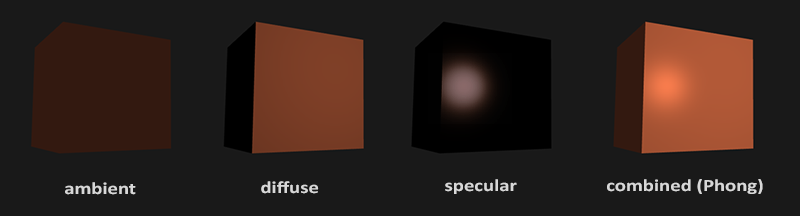
\includegraphics[width=1.0\textwidth]{images/phong_model.png}
		\caption{冯氏光照模型分量}
		\label{phong_model}
    \end{figure}
    
    \begin{itemize}
    	\item 环境光照(Ambient Lighting):即使在黑暗的情况下,世界上通常也仍然有一些光亮(月亮、远处的光),所以物体几乎永远不会是完全黑暗的。为了模拟这个,我们会使用一个环境光照常量,它永远会给物体一些颜色。
    	\item 漫反射光照(Diffuse Lighting):模拟光源对物体的方向性影响(Directional Impact)。它是冯氏光照模型中视觉上最显著的分量。物体的某一部分越是正对着光源,它就会越亮。
    	\item 镜面光照(Specular Lighting):模拟有光泽物体上面出现的亮点。镜面光照的颜色相比于物体的颜色会更倾向于光的颜色。
    \end{itemize}
    
    将上述三个分量全部叠加后即可得到最终的渲染颜色。
    
    \subsection{环境光照}
    
    在现实环境中,光源可能有很多个,并可能通过多个物体进行反射从而简介对其他物体产生影响。考虑到这种情况的算法叫全局光照(Global Illumination)算法,但是这种算法开销极高,且运算较为复杂。\\
    在冯氏光照中采用了最简单的方法模拟环境光照,即用常量因子乘以环境颜色获得一个近似结果,它在代码中的体现如下:
   
   
	\begin{lstlisting}[language={[ANSI]C},numbers=left,numberstyle=\tiny,%frame=shadowbox,
   rulesepcolor=\color{red!20!green!20!blue!20},
   keywordstyle=\color{blue!70!black},
   commentstyle=\color{blue!90!},
   basicstyle=\ttfamily]
	Color PhongShader::getAmbient(const VertexOut &frag) const {
    Color ambient = _ambient.color * _ambient.factor;
    return ambient;
	}
	\end{lstlisting}
	
	\subsection{漫反射光照}
	
	比起环境光照,漫反射光照分量最能产生显著的视觉影响。它的思想是,同光线角度最接近的片段可以获得最高的亮度:
	
	\begin{figure}[H]
    	\centering
		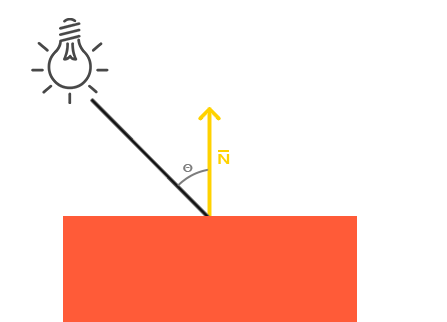
\includegraphics[width=1.0\textwidth]{images/diffuse_light.png}
		\caption{漫反射分量示意图}
		\label{diffuse_light}
    \end{figure}
	
	如图,其中$\overline N$代表其中一个片元的法向量,它与光照方向产生了角度$\theta$;对光线入射向量和法向量分别标准化,之后取两者的点积可以得到$cos\theta$,将该值与光线颜色相乘,取一个比例系数之后得到结果,该值的大小反映了夹角大小的同时也指代了光线的明暗。\\
	值得注意的是,有时候这个点积会得到负值,但这意味着光线与某个法向量成钝角,也就是在片元的“另一边”,此时在实现时只需要将它取为0即可,下面是漫反射分量在代码中的体现:
	
	\begin{lstlisting}[language={[ANSI]C},numbers=left,numberstyle=\tiny,%frame=shadowbox,
   rulesepcolor=\color{red!20!green!20!blue!20},
   keywordstyle=\color{blue!70!black},
   commentstyle=\color{blue!90!},
   basicstyle=\ttfamily]
	double cosTheta = ray.dot(normal);
    double diff = max(cosTheta , (double)0.0f);
    Color diffuse = _light.color* _light.factor * diff * _material.diffuseFactor;
    return diffuse;
	\end{lstlisting}
	
	\subsection{镜面光照}
	
	镜面光照将观察者的观察向量也融入到了渲染之中。假设物体是一面镜子,那么入射的光将被完全反射,此时就必须考虑该反射光和观察者视角对于物体亮度的影响。
	
    \begin{figure}[H]
    	\centering
		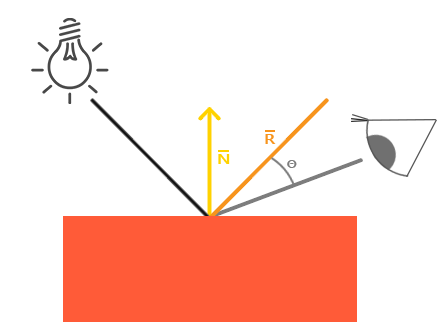
\includegraphics[width=1.0\textwidth]{images/specular_light.png}
		\caption{镜面分量示意图}
		\label{specular_light}
    \end{figure}
    
    如图,我们通过反射法向量周围光的方向来计算反射向量。然后我们计算反射向量和视线方向的角度差,如果夹角越小,那么镜面光的影响就会越大。它的作用效果就是,当我们去看光被物体所反射的那个方向的时候,我们会看到一个高光,它的代码实现如下:
    \begin{lstlisting}[language={[ANSI]C},numbers=left,numberstyle=\tiny,%frame=shadowbox,
   rulesepcolor=\color{red!20!green!20!blue!20},
   keywordstyle=\color{blue!70!black},
   commentstyle=\color{blue!90!},
   basicstyle=\ttfamily]
   Vec3 center = (ray + viewDir).getNormalize();
	 auto spec = pow(max(center.dot(normal), 0.0), _material.shininess);
    Color specular = _light.color * _light.factor * spec * _material.specularFactor;
    return specular;
	\end{lstlisting}
    
    在实现时,计算反射光的法向量比较麻烦,为此,先将入射光单位向量和观察方向单位向量相加求出两者的角平分线,之后再计算角平分线与法向量的夹角,这个计算的合理性如下:
   		\begin{equation}
   			\frac{2\alpha+\theta}{2} - \alpha = \frac{\theta}{2}
   		\end{equation}
    其中,$\alpha$是入射角,$\theta$是待求夹角。\\
    在下一行,将求得的值取了一个次幂,所取的指数叫做反光度(Shininess),一个物体的反光度越高,反射光的能力越强,散射得越少,高光点就会越小。下面的图片反映了不同反光度对渲染效果的影响:
    
    \begin{figure}[H]
    	\centering
		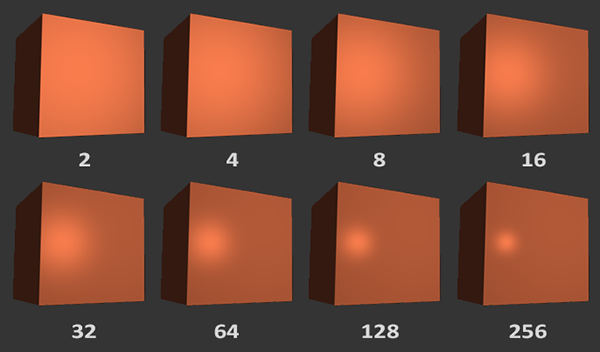
\includegraphics[width=1.0\textwidth]{images/shininess.png}
		\caption{不同反光度的视觉效果}
		\label{shininess}
    \end{figure}
    
    最后,将上述三个分量参数简单相加后乘以物体本身的颜色,即输出冯氏光照的结果。
    	
    \end{spacing}
  

    \section{三维模型}

        \begin{spacing}{2.5}
    三维模型的导入使用到了第三方assimp库,assimp是OpenGL的一个三维模型读取接口,通过这一接口可以读取常见的三维模型文件如obj文件。assimp的架构如下:
    \begin{figure}[H]
    	\centering
		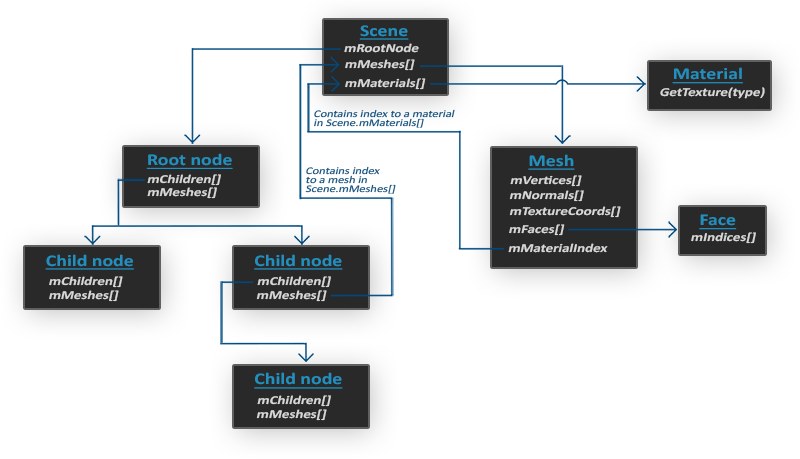
\includegraphics[width=1.0\textwidth]{images/assimp.png}
		\caption{Assimp的架构}
		\label{shininess}
    \end{figure}
    
    
    通过引入assimp包,我们就可以在代码中读取obj格式的三维模型,具体方式如下:
        \end{spacing}

    \begin{lstlisting}
void Sprite3D::init(const std::string &fileName) {
    _shader = Sprite3DShader::create();
    Assimp::Importer importer;
    const aiScene * scene = importer.ReadFile(getFullPath(fileName), aiProcess_Triangulate | aiProcess_FlipUVs);
    initShader();
    handleNode(scene->mRootNode , scene);
}	
    \end{lstlisting}

\begin{spacing}{2.5}
接下来是三维模型的获取,我们没有从网上直接找现成的三维模型,而是借助Photoshop和Maya,自己制作了一个同济大学校徽的三维模型,我们认为这样更有意义。
    \begin{figure}[H]
    	\centering
		
\includegraphics[width=0.8\textwidth]{images/tj-logo.png}
		\caption{校徽的三维模型}
		\label{shininess}
    \end{figure}
\end{spacing}


    \section{天空盒子}
            \begin{spacing}{2.5}
            	     在实时渲染中,如果要绘制非常远的物体,例如远处的山、天空等,随着观察者的距离的移动,这个物体的大小是几乎没有什么变化的,这个时候可以考虑采用天空盒子技术。
            \end{spacing}


     \begin{figure}[H]
    	\centering
		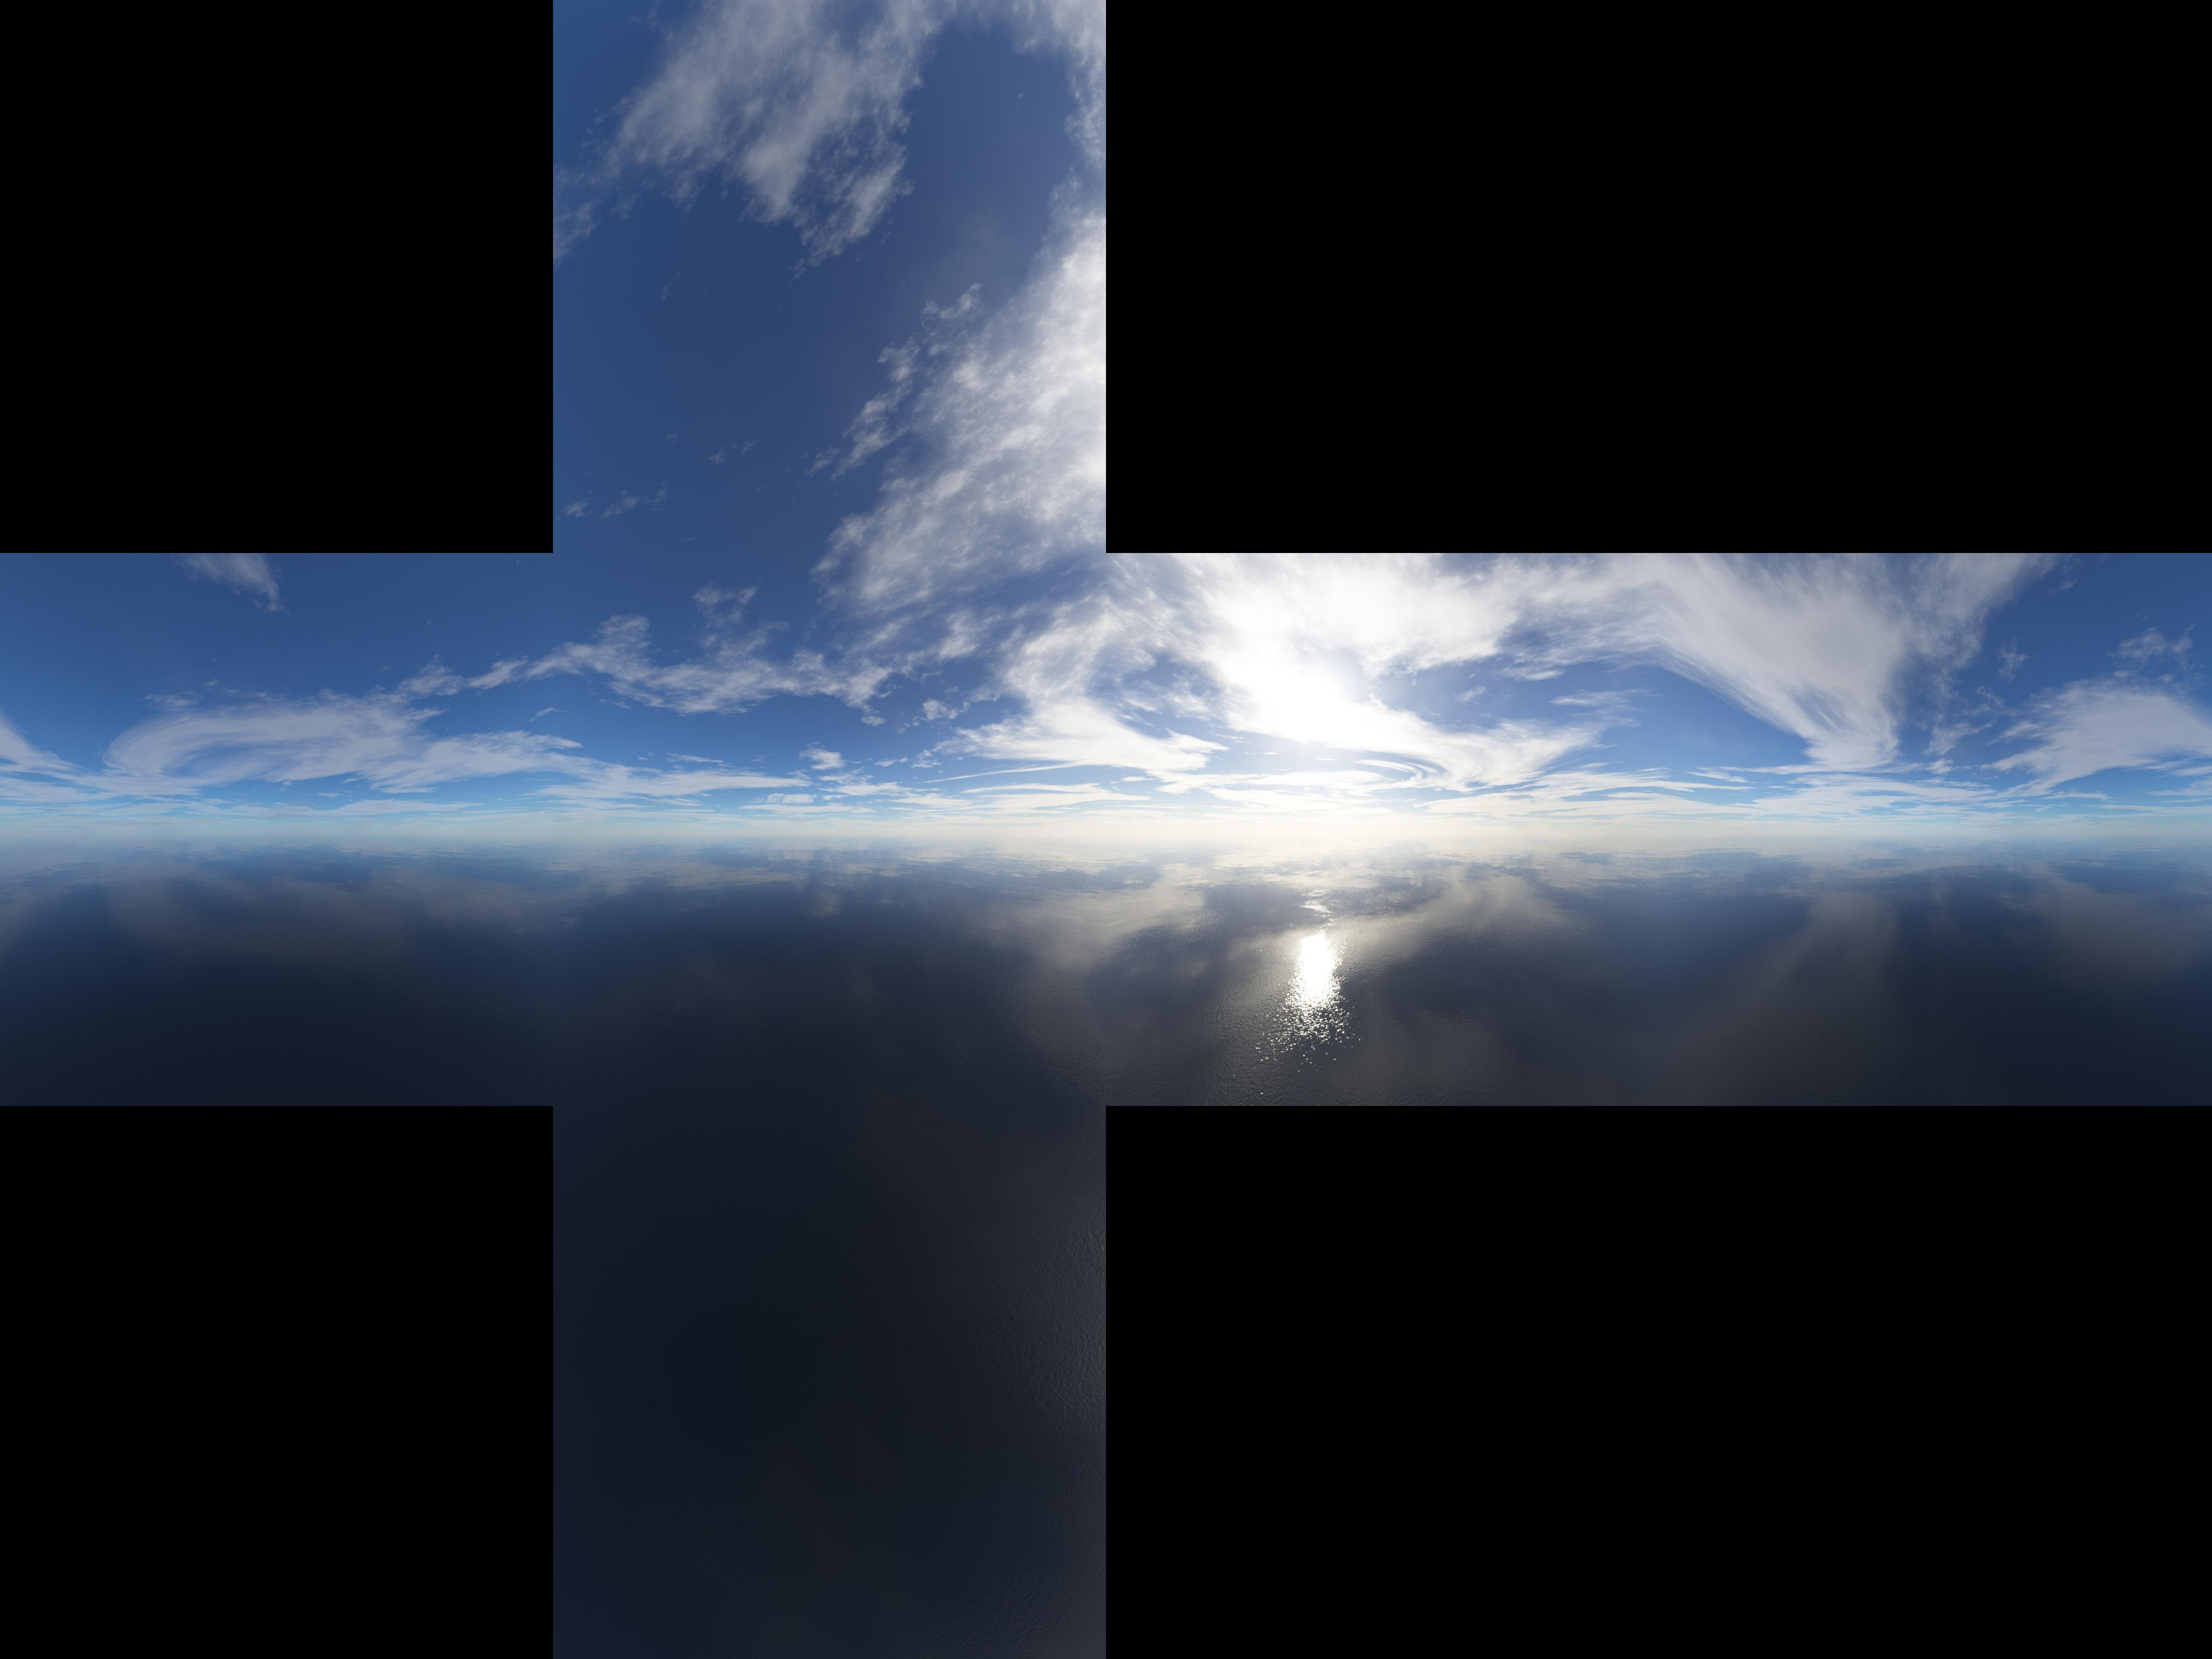
\includegraphics[width=1.0\textwidth]{images/skybox.jpeg}
		\caption{天空盒子示意图}
		\label{skybox}
    \end{figure}
                \begin{spacing}{2.5}
                	    如同,所谓的天空盒实际就是一个单位立方体展开,然后在六个面贴上相应的贴图即可。在实际实现时,将立方体的坐标指定为单位元。
                \end{spacing}


    
    
\end{document}
